% arara: pdflatex
% arara: bibtex
% arara: pdflatex
% arara: pdflatex
\documentclass{article}

\usepackage{graphicx}  % for including graphics
\usepackage{amsmath}   % math symbols like operator notation
\usepackage{siunitx}     % properly format quantities with units
\usepackage{fancyhdr}  % control headers
\usepackage{physics}
\usepackage{fullpage}

\title{Numerical Evaluation of the Arrhenius Integral}
\author{C.D. Clark III}


\begin{document}
\maketitle

The Arrhenius
Integral model for thermal damage requires the evaluation of the integral\cite{WELCH--2011--optical-thermalresponseoflaser-irradiatedtissue}
\begin{equation}
  \label{eqn:arr}
  \Omega\qty(\tau) = \int\limits_{0}^{\tau} A e^{\frac{-Ea}{RT\qty(t)}} dt.
\end{equation}
If the temperature, $T\qty(t)$, is predicted using a numerical simulation, i.e. a finite-difference or finite-element model, then the temperature is calculated at a discrete set of times, $(t_0, t_1,
\ldots)$. This limits the methods that can be used to evaluate Eq. \ref{eqn:arr} numerically to those that work on predefined nodes (Gaussian quadrature, for example, cannot be used).

The usual methods for numerically evaluating an integral with pre-defined nodes would be Reimann sum, Trapezoid Rule,
and Simpson's Rule. These methods are simple to implement, but approximate the integrand as piece-wise, linear, and
parabolic, respectivly.



\section{Recasting the integral}
If we assume that the temperature between two times, $t_0$ and $t_1$ can be written as a linear function of time,
\begin{equation}
  T\qty(t) = mt + T_0
\end{equation}
and inserting into this into Eq. \ref{eqn:arr} gives,
\begin{equation}
  \Omega = \int\limits_{t_0}^{t_1} A e^{\frac{-Ea}{R\left(mt + T_0\right)}} dt.
\end{equation}
Changing the integration variable to $T$,
\begin{align}
  dT &= mdt \\
  \Omega &= \int\limits_{T_0}^{T_1} \frac{A}{m}e^{\frac{-Ea}{RT}} dT.
\end{align}
Where $T_0$ and $T_1$ are the temperature at $t_0$ and $t_1$. Next, we substitute $u = \frac{E_a}{RT}$ and change the integration variable again to $u$.
\begin{align}
  u &= \frac{E_a}{R} \frac{1}{T}  \\
  du &= -\frac{E_a}{R} \frac{1}{T^{2}} dT  \\
  dT &= -\frac{E_a}{R} \frac{1}{u^{2}} du  \\
  \Omega &= -\frac{A}{m}\frac{E_a}{R} \int\limits_{E_a / R T_0}^{E_a / R T_1} \frac{e^{-u}}{u^2} du  \\
  \label{eqn:arr_2}
         &=  \frac{A}{m}\frac{E_a}{R} \int\limits_{E_a / R T_1}^{E_a / R T_0} \frac{e^{-u}}{u^2} du.
\end{align}
The integrand can be evaluated ``analytically'' using the \emph{exponential integral}, $E_n$, which is defined as\cite{1970--handbookofmathematicalfunctionswithformulas}
\begin{equation}
  E_n\qty(x) = \int\limits_{1}^{\infty} \frac{e^{-xt}}{t^n} dt
\end{equation}
The variable substitution $y = xt$ gives
\begin{align}
  dy &= xdt \\
  dt &= \frac{1}{x}dy \\
  E_n\qty(x) &= x\int\limits_{x}^{\infty} \frac{e^{-y}}{y^n} dy
\end{align}
Comparing this to Eq. \ref{eqn:arr_2}, it is simple to show that
\begin{align}
  \Omega &= \frac{A}{m}\frac{E_a}{R} \left[\frac{E_2\qty{E_a/RT_1}}{E_a/RT_1} - \frac{E_2\qty{E_a/RT_0}}{E_a/RT_0}\right] \\
         &= \frac{A}{m}              \left[T_1 E_2\qty{E_a/RT_1}              - T_0 E_2\qty{E_a/RT_0}             \right]
\end{align}
Finally, we note that the slope, $m$, can be determined from $T_0$ and $T_1$ if $t_1$ and $t_0$ are known (rise over run),
\begin{align}
  \Omega &= A \frac{t_1 - t_0}{T_1 - T_0}              \left[T_1 E_2\qty{E_a/RT_1}              - T_0 E_2\qty{E_a/RT_0}             \right]
\end{align}
This gives the accumulated damage over a time $t_1 - t_0$, when the temperature rise is linear. If the actual
temperature rise is not linear, then we can discretize the profile into small segments, such that
the temperature is approximatly linear over the segment. It is reasonalble to think that this approximation
(treating the temperature as linear over some time interval) is better than assuming that the damage rate
is linear over the same time. Figure \ref{fig:arrhenius_rate} shows the Arrhenius rate as a function of time for an example
thermal profile. The figure shows that the Arrhenius rate is concave on both sides its peak, which means that the error accumlated by the
trapezoid rule will have the same sign on each side. The trapezoid rule will \emph{over}-predict the accumulated damage. On the otherhand,
if the thermal profile is approimated as linear segments, the accumulated damage will be \emph{under}-predicted while the temperature increases, and
then be \emph{over}-predicted when the temperature begins to fall.


\begin{figure}
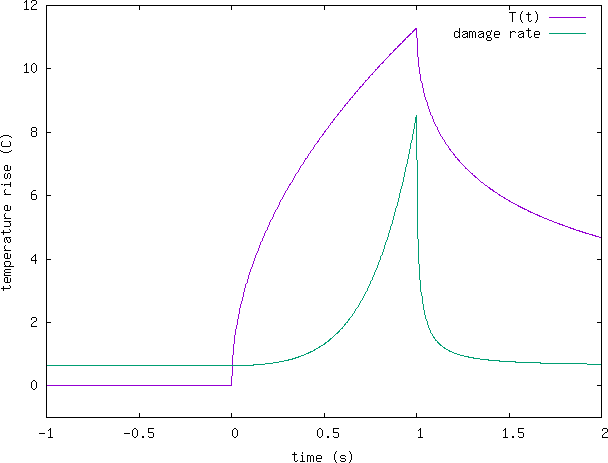
\includegraphics{./arrhenius_rate.png}
\caption{\label{fig:arrhenius_rate} The Arrhenius rate, $Ae^{-E_a/RT(t)}$, plotted for an example thermal profile. }
\end{figure}


\bibliography{references_database}
\bibliographystyle{plain}


\end{document}
